\documentclass{article}

% Needs to be loaded before cleveref, so we can specify the name
% of a `listing` environment (https://tex.stackexchange.com/a/47694)
\usepackage{listings}
%%% Local Variables:
%%% mode: latex
%%% TeX-master: "../main"
%%% End:

% Recommended, but optional, packages for figures and better typesetting:
\usepackage{microtype}
\usepackage{graphicx}
\usepackage{booktabs} % for professional tables

% hyperref makes hyperlinks in the resulting PDF.
% If your build breaks (sometimes temporarily if a hyperlink spans a page)
% please comment out the following usepackage line and replace
% \usepackage{icml2024} with \usepackage[nohyperref]{icml2024} above.
\usepackage{hyperref} % hyperlinks

% Attempt to make hyperref and algorithmic work together better:
\newcommand{\theHalgorithm}{\arabic{algorithm}}

% Use the following line for the initial blind version submitted for review:
% \usepackage{icml2024}

% If accepted, instead use the following line for the camera-ready submission:
\usepackage[accepted]{icml2024}

% For theorems and such
\usepackage{amsmath}
\usepackage{amssymb}
\usepackage{mathtools}
\usepackage{amsthm}

% if you use cleveref..
\usepackage[capitalize,noabbrev]{cleveref}

%%%%%%%%%%%%%%%%%%%%%%%%%%%%%%%%
% THEOREMS
%%%%%%%%%%%%%%%%%%%%%%%%%%%%%%%%
\theoremstyle{plain}
\newtheorem{theorem}{Theorem}[section]
\newtheorem{proposition}[theorem]{Proposition}
\newtheorem{lemma}[theorem]{Lemma}
\newtheorem{corollary}[theorem]{Corollary}
\theoremstyle{definition}
\newtheorem{definition}[theorem]{Definition}
\newtheorem{assumption}[theorem]{Assumption}
\newtheorem{example}[theorem]{Example}
\theoremstyle{remark}
\newtheorem{remark}[theorem]{Remark}
%%% Local Variables:
%%% mode: latex
%%% TeX-master: "../main"
%%% End:

\input{preamble/goodfellow.tex}
% ===================================================================
% WRITING
% ===================================================================
\usepackage{paracol}
\usepackage{blindtext}
\newcommand{\felix}[1]{\textcolor{red}{Felix: #1}}
\newcommand{\balint}[1]{\textcolor{orange}{Bálint: #1}}

% ===================================================================
% COLORS
% ===================================================================
% VECTOR PRIMARY COLORS
\definecolor{VectorBlack}{RGB}{34, 34, 34}
\definecolor{VectorGray}{RGB}{239, 238, 237}

% VECTOR SECONDARY COLORS
\definecolor{VectorBlue}{RGB}{59, 69, 227}
\definecolor{VectorPink}{RGB}{253, 8, 238}
\definecolor{VectorOrange}{RGB}{250, 173, 26}
\definecolor{VectorTeal}{RGB}{82, 199, 222}

% ===================================================================
% REFERENCES
% ===================================================================
\hypersetup{%
  colorlinks,
  citecolor = VectorBlue,%
  linkcolor = VectorBlue,%
  urlcolor = VectorPink,%
}%
% tell cleveref how to name a listing environment
\crefname{listing}{snippet}{snippets}
% Rename Listing into Snippet
\renewcommand{\lstlistingname}{Snippet}

% ===================================================================
% CODE BLOCKS
% ===================================================================
% define style for listings using the Vector color scheme
\lstdefinestyle{vector_institute}{
  backgroundcolor=\color{VectorGray!50},
  commentstyle=\bfseries\color{VectorBlue},
  keywordstyle=\bfseries\color{VectorBlack},
  numberstyle=\tiny\color{VectorBlack!50},
  stringstyle=\bfseries\color{VectorPink},
  basicstyle=\ttfamily\scriptsize,
  xleftmargin=3.2ex,
  breakatwhitespace=false,
  breaklines=true,
  captionpos=t,
  keepspaces=true,
  numbers=left,
  numbersep=7pt,
  showspaces=false,
  showstringspaces=false,
  showtabs=false,
  tabsize=2,
  escapebegin={\color{blue}},
  linewidth=\linewidth,
  mathescape=true,
}
% use the above style as default
\lstset{style=vector_institute}

\usepackage{caption}
% modify captions of code blocks
\captionsetup[lstlisting]{%
  font={scriptsize},%
  justification=raggedright,%
  singlelinecheck=false,%
}

% \usepackage{minted}
% \usemintedstyle{emacs}

\newcommand{\repourl}{https://github.com/f-dangel/kfac-from-scratch}
% Command to include code blocks and their output.
% First argument is the filename inside the kfac_tutorial directory.
% The listing can be referenced with that filename, too.
\newcommand{\codeblock}[1]{
  % convert _ into \_ for LaTeX
  \def\filename{\detokenize{#1}}
  % \inputminted[%
  % fontsize=\scriptsize,%
  % % obeytabs,%
  % tabsize=0,%
  % bgcolor=VectorGray!50,%
  % texcomments=true,%
  % ]{python}{../kfs/#1.py}
  \lstinputlisting[%
  language=python,%
  caption=\href{\repourl/kfs/#1.py}{\texttt{kfs/\filename.py}},%
  label=#1,%
  ]{../kfs/#1.py}
  % \vspace{-1.25\baselineskip}
  % \lstinputlisting[%
  % language=python,%
  % numbers=none,%
  % basicstyle=\bfseries\ttfamily\scriptsize,%
  % title=\href{\repourl/tex/output/#1.txt}{Output:}\hfill,%
  % ]{output/#1.txt}
}

% ===================================================================
% MATH
% ===================================================================
\usepackage{nicefrac}
\DeclareMathOperator{\rvec}{rvec}
\DeclareMathOperator{\cvec}{cvec}
\let\vec\relax % delete the existing \vec command
\DeclareMathOperator{\vec}{vec}
\DeclareMathOperator{\mat}{mat}
\DeclareMathOperator{\lin}{lin}

\usepackage{mdframed}
\mdfdefinestyle{custom}{%
  linecolor=black,%
  topline=false,%
  bottomline=false,%
  rightline=false,%
  linewidth=1.25pt,%
  backgroundcolor=VectorGray!50,%
  innerleftmargin=5pt,%
  % innertopmargin=8pt,%
}
\theoremstyle{definition}
\newmdtheoremenv[style=custom]{definition}{Definition}[section]
\newmdtheoremenv[style=custom]{setup}{Setup}[section]
\newmdtheoremenv[%
style=custom,%
linecolor=VectorOrange,%
backgroundcolor=VectorOrange!10,%
]{caveat}{Caveat}[section]
\newmdtheoremenv[%
style=custom,%
linecolor=VectorTeal,%
backgroundcolor=VectorTeal!10,%
]{test}{Test}[section]
\newmdtheoremenv[%
style=custom,%
linecolor=VectorTeal,%
backgroundcolor=VectorTeal!10,%
]{example}{Example}[section]

% ===================================================================
% FIGURES
% ===================================================================
\usepackage{tikz}
\usetikzlibrary{arrows.meta}
\usetikzlibrary{positioning}

%%% Local Variables:
%%% mode: latex
%%% TeX-master: "../main"
%%% End:


\begin{document}

\onecolumn
\newcommand{\papertitle}{%
  Kronecker-factored Approximate Curvature (KFAC) From Scratch
}%
\title{\papertitle}

% The \icmltitle you define below is probably too long as a header.
% Therefore, a short form for the running title is supplied here:
\icmltitlerunning{\papertitle}

\icmltitle{\papertitle}

% It is OKAY to include author information, even for blind
% submissions: the style file will automatically remove it for you
% unless you've provided the [accepted] option to the icml2024
% package.

% List of affiliations: The first argument should be a (short)
% identifier you will use later to specify author affiliations
% Academic affiliations should list Department, University, City, Region, Country
% Industry affiliations should list Company, City, Region, Country

% You can specify symbols, otherwise they are numbered in order.
% Ideally, you should not use this facility. Affiliations will be numbered
% in order of appearance and this is the preferred way.
\icmlsetsymbol{equal}{*}

\begin{icmlauthorlist}
\icmlauthor{Felix Dangel}{equal,vector}
\icmlauthor{Runa Eschenhagen}{equal,cambridge}
\icmlauthor{B\'alint Mucs\'anyi}{equal,tue}
\icmlauthor{Tobias Weber}{equal,tue}
\end{icmlauthorlist}

\icmlaffiliation{vector}{Vector Institute, Canada}
\icmlaffiliation{cambridge}{University of Cambridge, United Kingdom}
\icmlaffiliation{tue}{University of T\"ubingen, Germany}

\icmlcorrespondingauthor{Felix Dangel}{fdangel@vectorinstitute.ai}
% \icmlcorrespondingauthor{Firstname2 Lastname2}{first2.last2@www.uk}

% You may provide any keywords that you
% find helpful for describing your paper; these are used to populate
% the "keywords" metadata in the PDF but will not be shown in the document
\icmlkeywords{KFAC, Natural gradient descent}

\vskip 0.3in

% this must go after the closing bracket ] following \twocolumn[ ...

% This command actually creates the footnote in the first column
% listing the affiliations and the copyright notice.
% The command takes one argument, which is text to display at the start of the footnote.
% The \icmlEqualContribution command is standard text for equal contribution.
% Remove it (just {}) if you do not need this facility.

% \printAffiliationsAndNotice{}  % leave blank if no need to mention equal contribution
\printAffiliationsAndNotice{\icmlEqualContribution} % otherwise use the standard text.
%%% Local Variables:
%%% mode: latex
%%% TeX-master: "../main"
%%% End:
 % Creates title

\vspace*{-2ex}

% logo
\begin{center}
\begin{tikzpicture}
    \node[inner sep=0.7pt, opacity=0.5, draw opacity=1, draw=black!50!white, ultra thick, rounded corners]{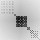
\includegraphics[scale=0.66]{figures/logo.pdf}};
\end{tikzpicture}
\end{center}

\vfill

\begin{abstract}
  Kronecker-factored approximate curvature \citep[KFAC,][]{martens2015optimizing} is arguably one of the most prominent curvature approximations in deep learning.
  Its applications range from optimization to Bayesian deep learning, training data attribution with influence functions, and model compression or merging.
  While the intuition behind KFAC is easy to understand, its implementation is tedious: It comes in many flavours, has common pitfalls when translating the math to code, and is challenging to test, which complicates ensuring a properly functioning implementation.
  Some of the authors themselves have dealt with these challenges and experienced the discomfort of not being able to fully test their code.
  Thanks to recent advances in understanding KFAC, we are now able to provide test cases and a recipe for a reliable KFAC implementation.
  \emph{This tutorial is meant as a ground-up introduction to KFAC.}
  In contrast to the existing work, our focus lies on providing both math and code side-by-side and providing test cases based on the latest insights into KFAC that are scattered throughout the literature.
  We hope this tutorial provides a contemporary view of KFAC that
  allows beginners to gain a deeper understanding of this curvature approximation while lowering the barrier to its implementation, extension, and usage in practice.
\end{abstract}

\vfill

\paragraph{Version:} \today\,(v1.0.0)

\paragraph{About the length of this document.}
Before you close this document because you saw the page count:
the \emph{effective length is much shorter than suggested by its page number}.
This is because \emph{we use an experimental two-column layout which presents text and code in parallel} and leads to a large amount of white space.
The left column contains the main text with explanations and mathematical descriptions.
The right column accompanies the left one with code snippets to make the ideas precise in code; it can safely be skipped if you are in a rush.
And if you already know the basics, it suffices to read the KFAC-specific part (Pages \pageref{sec:kfac-overview}--\pageref{sec:kfac-cheatsheet}).

\paragraph{Follow along in code.} The \LaTeX\,\& Python source code is available at~\href{\repourl}{\texttt{github.com/f-dangel/kfac-tutorial}}.
This allows you to run the code as you read:
Clone the repository and follow the installation instructions.
You can then run each snippet from the repository root, for instance by calling \texttt{python kfs/basics/forward\_pass.py}.
If you find typos or have suggestions for improving explanations, math, or code, please open issues and pull requests.
In doing so, you are contributing to making this tutorial a valuable reference for newcomers.

\vspace{\baselineskip}
%%% Local Variables:
%%% mode: latex
%%% TeX-master: "../main"
%%% End:

\clearpage

\tableofcontents
\clearpage

\section{Preface}
This is an attempt to bundle scattered knowledge about KFAC into a single document, explain all the technicalities and pitfalls, and present tests to ensure bug-free implementations.

Should answer the following questions:
\begin{itemize}
\item Why do we need this tutorial?
\item Why is this not a Jupyter notebook?
\item What do we gain by explaining KFAC bottom-up?
\item What ML framework do we use and why?
\item What are we \emph{not} doing (e.g.\,building an optimizer)?
\end{itemize}

We use PyTorch~\cite{paszke2019pytorch} and implement everything using \texttt{torch.nn} rather than a functional formulation as we feel that many deep learning practitioners are more familiar with this style.
There could be a JAX or functorch version, too.

\begin{itemize}
\item KFAC approximates the Fisher, which is an outer product of gradients. The gradients involve the output-parameter Jacobian of a weight, which has Kronecker structure,
  \begin{align}
    \jac_{\mW}(\mW \vx) = \vx^{\top} \otimes \mI\,.
  \end{align}
  This implies that the Fisher contains terms of the following form, where $\bullet$ is a placeholder for some matrix,
  \begin{align}
    \left(
    \vx^{\top}\otimes \mI
    \right)^{\top}
    \bullet
    \left(
    \vx^{\top}\otimes \mI
    \right)\,.
  \end{align}

\item The goal is to build up to an abstract general formulation of KFAC.
  Given a compute graph which uses the operations $\vx, \mW \mapsto \mW x$, potentially in multiple places, define a Kronecker approximation of the Fisher.
  Also to show the different degrees of freedom: treating weights \& biases jointly/separately, using reduce versus expand approximation, and treating weight tying, i.e.
  multi-usage of $\mW$.

\end{itemize}
TODO Should mention somewhere that many of the provided examples are already discussed in Felix's PhD thesis~\cite{dangel2023backpropagation}.

\paragraph{KFAC flavours} There are various degrees of freedom that induce different KFAC flavours:
\begin{align*}
  \begin{array}{c}
    \begin{Bmatrix}
      \text{PyTorch}
      \\
      \text{JAX}
    \end{Bmatrix}
    \\
    \text{(software framework)}
  \end{array}
  \times
  \begin{array}{c}
    \begin{Bmatrix}
      \rvec
      \\
      \cvec
    \end{Bmatrix}
    \\
    \text{(flattening convention)}
  \end{array}
  \times
  \begin{array}{c}
    \begin{Bmatrix}
      \text{MC (type-I Fisher)}
      \\
      \text{type-II Fisher}
      \\
      \text{empirical Fisher}
    \end{Bmatrix}
    \\
    \text{(target curvature)}
  \end{array}
  \times
  \begin{array}{c}
    \begin{Bmatrix}
      \text{expand}
      \\
      \text{reduce}
    \end{Bmatrix}
    \\
    \text{(how weight sharing is handled)}
  \end{array}
  \times
  \begin{array}{c}
    \begin{Bmatrix}
      \text{fully-connected}
      \\
      \text{convolutions}
    \end{Bmatrix}
    \\
    \text{(layers)}
  \end{array}
\end{align*}
The original work from~\citet{martens2015optimizing} uses
\begin{align*}
  \text{cvec} \times \text{MC (type-I Fisher)} \times \text{expand} \times \text{fully-connected}\,.
\end{align*}
\paragraph{Version 1.0} This document aims to provide an introduction to the following flavours:
\begin{align*}
  \text{PyTorch}
  \times
  \begin{Bmatrix}
    \rvec
    \\
    \cvec
  \end{Bmatrix}
  \times
  \begin{Bmatrix}
    \text{MC (type-I Fisher)}
    \\
    \text{type-II Fisher}
    \\
    \text{empirical Fisher}
  \end{Bmatrix}
  \times
  \text{expand}
  \times
  \text{fully-connected}
\end{align*}
This allows us to (i) highlight challenges when translating math to code, (ii) pointing out various connections between the curvature matrices and KFAC, and (iii) produce a working, tested, version of the original KFAC paper with slight generalizations.
%%% Local Variables:
%%% mode: latex
%%% TeX-master: "../main"
%%% End:

\clearpage

\columnratio{0.42}
\begin{paracol}{2}
  \section{Basics}
  \subsection{Empirical risk minimization \& Maximum Likelihood Estimation}

\begin{paracol}{2}

  \begin{align}
    \gL(\vtheta) &= \sum_{n=1}^N \ell(\vtheta, \vx_n, \vy_n)
    \\
                 &=
                   \sum_{n=1}^N c(f(\vtheta, \vx_n), \vy_n)
  \end{align}

  \switchcolumn[0]

  \blindtext

  \switchcolumn[1]

  \switchcolumn[0]* % sync

  \blindtext

  \switchcolumn[1]

  \codeblockWithOutput{hello_world}

  \switchcolumn[0]

  \Cref{hello_world} says hello world.

  \subsection{Derivatives}

  \begin{caveat}
    In deep learning, we often work with matrices, or higher-dimensional tensors.
    We want to use matrix linear algebra expressions to avoid using heavy index notation.
    This can be achieved by flattening all tensors back into vectors and re-using definitions derivatives from the vector case.
    However, we must be careful when translating the results back to the tensor format, as the translation process depends on the flattening convention.
    Classically, the mathematical derivations prefer a \emph{different} flattening scheme than the one used in deep learning libraries.
  \end{caveat}

  \switchcolumn[0]*
  \subsubsection{Flattening}

  There are two popular flattening conventions: last-varies-fastest and first-varies-fastest.

  \begin{example}
    For matrix
    \(
    \mA = \begin{pmatrix}
            1 & 2 \\
            3 & 4
          \end{pmatrix}
          \), we have
          \begin{equation*}
            \rvec(\mA)
            =
            \begin{pmatrix}
              1 \\ 2 \\ 3 \\ 4
            \end{pmatrix}\,,
            \qquad
            \cvec(\mA)
            =
            \begin{pmatrix}
              1 \\ 3 \\ 2 \\ 4
            \end{pmatrix}\,,
          \end{equation*}
          see \Cref{flattening}.
        \end{example}

        \switchcolumn[1]
        \codeblockWithOutput{flattening}

        \switchcolumn[0]*
        \subsubsection{Jacobians, JVP, VJPs}

        \begin{definition}[Jacobian]
          Consider a vector-to-vector function $f: \sR^A \to \sR^B, \va \mapsto \vb = f(\va)$.
          Its Jacobian $\jac_{\va}\vb \in \sR^{\mB \times \mA}$ collects the first-order partial derivatives into a matrix such that
          \begin{align*}
            [\jac_{\va} \vb]_{i,j} = \frac{\partial [f(\va)]_i}{\partial [\va]_j}\,.
          \end{align*}
        \end{definition}

        \begin{definition}[General Jacobian]
          TODO
        \end{definition}

        \begin{definition}[Vector-Jacobian products]
          TODO
        \end{definition}

        \begin{definition}[$\cvec$-Jacobian]
          Consider a tensor-to-tensor function $f: \sR^{A_1 \times \dots \times A_N} \to \sR^{B_1 \times \dots \times B_M}, \tA \mapsto \tB = f(\tA)$. Its $\cvec$-Jacobian $\jac^{\cvec}_{\tA}\tB \in \sR^{A_N \cdots A_1 \times B_M \cdots B_1}$ results from flattening input and output tensors with $\cvec$ and applying the Jacobian definition for vectors,
          \begin{align*}
            [\jac^{\cvec}_{\tA}\tB]_{i,j}
            =
            \frac{\partial [\cvec(f(\tA))]_i}{\partial [\cvec(\tA)]_j}\,.
          \end{align*}
        \end{definition}

        \begin{definition}[$\rvec$-Jacobian]
          Consider a tensor-to-tensor function $f: \sR^{A_1 \times \dots \times A_N} \to \sR^{B_1 \times \dots \times B_M}, \tA \mapsto \tB = f(\tA)$. Its $\cvec$-Jacobian $\jac^{\cvec}_{\tA}\tB \in \sR^{A_1 \cdots A_N \times B_1 \cdots B_M}$ results from flattening input and output tensors with $\cvec$ and applying the Jacobian definition for vectors,
          \begin{align*}
            [\jac^{\cvec}_{\tA}\tB]_{i,j}
            =
            \frac{\partial [\cvec(f(\tA))]_i}{\partial [\cvec(\tA)]_j}\,.
          \end{align*}
        \end{definition}

        \switchcolumn[1]
        \codeblockWithOutput{jacobians}


        \switchcolumn[1]*
        \codeblockWithOutput{jacobians_linear_layer}
        \switchcolumn[0]

        \begin{example}[$\cvec$- and $\rvec$-weight Jacobians of a linear layer]
          Consider an affine map with weight matrix $\mW \in \sR^{D_{\text{out}} \times D_{\text{in}}}$, bias vector $\vb \in \sR^{D_{\text{out}}}$, input vector $\vx \in \sR^{D_{\text{in}}}$ and output vector $\vz \in \sR^{D_{\text{out}}}$ with
          \begin{align*}
            \vz
            \coloneqq
            \mW \vx + \vb
            =
            \begin{pmatrix}
              \mW & \vb
            \end{pmatrix}
            \begin{pmatrix}
              \vx \\ 1
            \end{pmatrix}
            \coloneqq
            \tilde{\mW}
            \tilde{\vx}\,.
          \end{align*}
          To express this operation as matrix-vector multiplication, we combined weight and bias into a single matrix $\tilde{\mW}$ and augment the input with a one, yielding $\tilde{\vx}$, to account for the bias contribution.

          The $\cvec$-Jacobian w.r.t.\,the combined weight is
          \begin{align*}
            \jac^{\cvec}_{\tilde{\mW}}\vz
            =
            \tilde{\vx}^{\top}
            \otimes
            \mI_{D_{\text{out}}}\,.
          \end{align*}
          In contrast, the $\rvec$-Jacobian is
          \begin{align*}
            \jac^{\cvec}_{\tilde{\mW}}\vz
            =
            \mI_{D_{\text{out}}}
            \otimes
            \tilde{\vx}^{top}\,,
          \end{align*}
          see \Cref{jacobians_linear_layer}.
          Note that the order of Kronecker factors is \emph{reversed}, depending on the flattening scheme.
        \end{example}

        \begin{example}[$\cvec$- and $\rvec$-weight Jacobians of a linear layer with weight sharing]
          Consider the same affine map from above, but now processing multiple input vectors $\mX = \begin{pmatrix}\vx_1 & \dots & \vx_S\end{pmatrix} \in \sR^{D_{\text{in}}\times S}$, yielding a sequence $\mZ = \begin{pmatrix} \vz_1 & \dots & \vz_S\end{pmatrix} \in \sR^{D_{\text{out}}\times S}$ where each $\vz_s$ is produced like above.
          The parameters are \emph{shared} over all vectors in the input sequence.
          In matrix notation,
          \begin{align*}
            \mZ
            \coloneqq
            \mW \mX + \vb \vone^{\top}_S
            =
            \begin{pmatrix}
              \mW & \vb
            \end{pmatrix}
            \begin{pmatrix}
              \mX \\ \vone^{\top}_S
            \end{pmatrix}
            \coloneqq
            \tilde{\mW}
            \tilde{\mX}\,.
          \end{align*}
          The $\cvec$-Jacobian w.r.t.\,the combined weight is
          \begin{align*}
            \jac^{\cvec}_{\tilde{\mW}}\mZ
            =
            \tilde{\mX}
            \otimes
            \mI_{D_{\text{out}}}\,.
          \end{align*}
          In contrast, the $\rvec$-Jacobian is
          \begin{align*}
            \jac^{\cvec}_{\tilde{\mW}}\mZ
            =
            \mI_{D_{\text{out}}}
            \otimes
            \tilde{\mX}\,,
          \end{align*}
          see \Cref{jacobians_shared_linear_layer}.
        \end{example}

        \switchcolumn[1]
        \codeblockWithOutput{jacobians_shared_linear_layer}

      \end{paracol}
      \subsubsection{Hessians, HVPs}

      \subsection{Curvature Matrices}
      \subsubsection{The Generalized Gauss-Newton (GGN)}
      \subsubsection{The Fisher}
      \subsubsection{The Connection between GGN \& Fisher}
      \subsubsection{The Empirical Fisher (EF)}

      %%% Local Variables:
      %%% mode: latex
      %%% TeX-master: "../main"
      %%% End:


  \switchcolumn[0]*
  \section{KFAC for Linear Layers}
  The goal of this section should be to describe the KFAC approximation from~\cite{martens2015optimizing}
  \begin{test}[KFAC]
    Describe setting in which KFAC becomes exact.
  \end{test}

  \section{KFAC for Convolution Layers}
  The goal of this section should be to describe the KFAC approximation from~\cite{grosse2016kroneckerfactored}

  \section{KFAC for Linear Layers with Weight Sharing (expand and reduce)}
  The goal of this section should be to describe the unification from~\cite{eschenhagen2023kroneckerfactored}

  \section{Other aspects}
  \subsection{Weight tying, RNNs, PINNs}
  \subsection{Unnormalized densities}
  \subsection{KFAC for diffusion models}

\end{paracol}

\clearpage
{\footnotesize
  \bibliographystyle{icml2024.bst}
  \bibliography{references.bib}
}
%%% Local Variables:
%%% mode: latex
%%% TeX-master: "../main"
%%% End:


\appendix

\section{Important Loss Function Hessians and Their Symmetric Factorization}\label{app:loss_function_hessians}
TODO Write down the Hessian of BCEWithLogitsLoss.
%%% Local Variables:
%%% mode: latex
%%% TeX-master: "../main"
%%% End:


\end{document}

%%% Local Variables:
%%% mode: latex
%%% TeX-master: t
%%% End:
